\documentclass[10pt]{article}
\usepackage[margin=.75in]{geometry}
\usepackage[T1]{fontenc}
\usepackage{amsmath,amssymb,booktabs,longtable,hyperref,tikz}
\usetikzlibrary{arrows.meta,positioning}
\title{The 40-Ary Fractal Photonic Holonet\\Executable Interconnect, Gateway Ports and Measurement Blueprint}
\author{W33-Theory Engineering}
\date{23 October 2026 -- Logical architecture release}
\begin{document}\maketitle
\begin{abstract}
We turn the recursive 40-site Holonet description into two explicit graphs and a reusable 960-link 40-child parent interface. A four-point isotropic W33 line acts as a gateway set, naturally balancing nine non-gateway clients at each point. A Cartesian alternative spends more links for shorter routes. These are verified logical networks; no foundry-qualified optical switch, fabricated device, measured delay or quantum advantage is claimed.
\end{abstract}
\tableofcontents
\section{Paper and code provenance}
Reviewed sources include \texttt{holonet\_machine\_blueprint.pdf} (268 pages),
\texttt{photonic\_holonet.pdf} (351 pages), \texttt{holonet\_practical\_implications.pdf} (23 pages),
\texttt{papers/forty\_points/main.pdf} (203 pages at the audit snapshot),
and \texttt{docs/holonet\_machine\_blueprint.pdf} (38 pages).
Page/topic hashes are in \texttt{analysis/2026\_10\_23\_fractal\_source\_pdf\_audit.json}.
BT827 states a 40-ary recursion and a chart-aware $8n$ route bound; the Fractal MicroVM runtime already implements nested state and Cartesian routing. Holotrade's level-two analysis distinguished Cartesian, lexicographic and four-line gateway constructions. Pass 2686 explicitly withdrew the old ternary RTL circuit as a faithful physical Holonet model. Here we implement a specific matched-port hierarchy through arbitrary depth.
\section{Symplectic geometry and a gateway line}
Canonical rays in $\mathbb F_3^4$ are adjacent exactly when
\[
\langle u,v\rangle=u_0v_1-u_1v_0+u_2v_3-u_3v_2=0\pmod3.
\]
The resulting $\operatorname{SRG}(40,12,2,4)$ has 240 edges. A four-point totally isotropic line $L$ is a clique and a dominating set: every point outside $L$ is adjacent to exactly one line point; each line point serves exactly nine outside clients. Select an anchor $z\in L$.
\section{Two distinct fractal graphs}
Each depth-$n$ leaf address is $a=(a_0,\ldots,a_{n-1})\in\{0,\dots,39\}^n$.
\subsection{Four-gateway hierarchy $F_n$}
A legal hop changes precisely one digit $i$ along a W33 edge. For the innermost digit, no additional restriction applies. For higher digits the suffix must equal $(g,z,\dots,z)$ with $g\in L$. Every parent has 240 W33 child-pair edges, with four matched gateway links per edge: 960 undirected logical inter-child connections. Every child therefore has $4\times12=48$ partner-specific logical terminations. An actual optical implementation still requires a switch, multiplexing or dedicated parallel link hardware.
\subsection{Cartesian overlay $C_n$}
Any coordinate may change along a W33 edge, with no gateway-suffix constraint. This Cartesian power has degree $12n$ and exact diameter $2n$; it is more uniform but requires more interconnect links.
\subsection{A proved route without a global table}
Find the first differing source/target digit. Zero the remaining source suffix from deepest to shallowest along W33 paths of length at most two; cross the differing digit while the suffix is the designated gateway anchor; then fill destination suffix shallowest to deepest. Every hop is a legal graph edge. Therefore the constructed $F_n$ route has at most $4n-2$ hops. This graph-hop bound is not the same unit as the paper's separate chart/cube/apartment $8n$ budget and is not a photon latency measurement.
\begin{center}
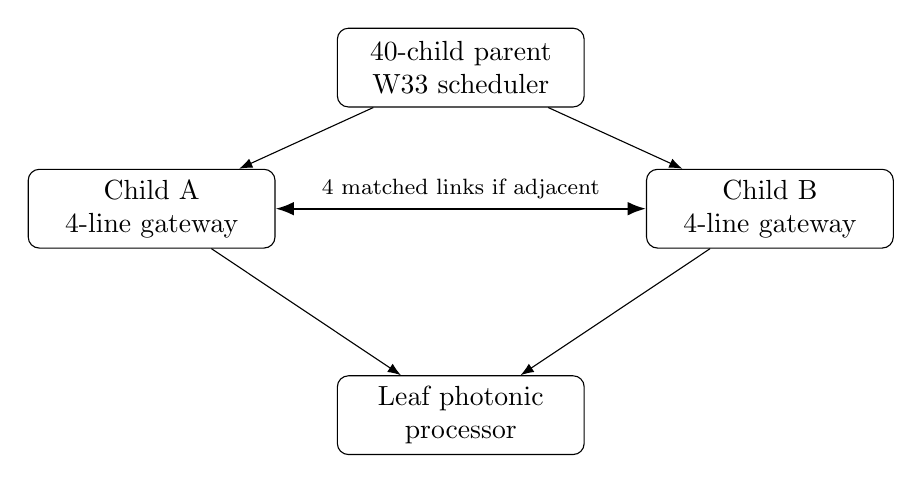
\begin{tikzpicture}[>=Latex,node distance=11mm,blk/.style={draw,rounded corners,minimum height=10mm,text width=29mm,align=center}]
\node[blk](p){40-child parent\\W33 scheduler};
\node[blk,below left=of p](a){Child A\\4-line gateway};
\node[blk,below right=of p](b){Child B\\4-line gateway};
\node[blk,below=of p,yshift=-23mm](core){Leaf photonic\\processor};
\draw[->](p)--(a);\draw[->](p)--(b);\draw[<->,thick](a)--node[above,sloped,font=\footnotesize]{4 matched links if adjacent}(b);
\draw[->](a)--(core);\draw[->](b)--(core);
\end{tikzpicture}
\end{center}
\section{Exact resource counts}
The number of W33 instances is $I_n=(40^n-1)/39$. Counting 240 links in each innermost W33 copy and 960 inter-child links at each higher parent yields
\[
E_F(n)=240\,40^{n-1}+960\frac{40^{n-1}-1}{39},
\quad E_C(n)=240n40^{n-1}.
\]
\begin{center}\begin{tabular}{rrrrrr}\toprule
Depth&Leaves&Instances&$F_n$ links&$C_n$ links&Diameters\\\midrule
1&40&1&240&240&(2,2) exact\\
2&1600&41&10560&19200&(5,4) exact BFS\\
3&64000&1641&423360&1152000&($\le 10$,6)\\\bottomrule
\end{tabular}\end{center}
Full BFS from all 1600 depth-two sources proves gateway diameter 5, with 160 vertices of eccentricity 4 and 1440 of eccentricity 5; Cartesian diameter is exactly 4. The level-three gateway diameter has only the constructive upper bound stated here.
\section{Hardware interface and falsification plan}
\begin{longtable}{p{.24\linewidth}p{.38\linewidth}p{.26\linewidth}}\toprule
Module&Logic ports&Physical work still open\\\midrule
W33 leaf tile&40 node addresses, 240 base adjacency links&device and waveguide design\\
Parent router&40 child instances, 960 matched links&optical switching and packaging\\
Gateway line&4 line lanes, 12 peer links per lane&contention, link arbitration\\
Parent endpoints&1920 directional port descriptions&duplex design, optical fanout\\
Photonic processor&independent 16-mode compiled unitary&not itself a 48-link switch\\
Controller&route requests, ACKs, timestamps&RTL scheduling and hardware clocks\\
Measurements&herald, transmission, timing, error, crosstalk&actual calibrated optical bench\\\bottomrule
\end{longtable}
A test must (i) verify each selected route against geometric adjacency, (ii) measure switch contention and failed links, (iii) extract optical S-parameters and loss and (iv) establish physical routing/PDK/DRC and package compliance. Finite graph geometry cannot prove photonic fidelity, noise tolerance, scalable quantum gates, or fabricated network reliability.
\section{Reproducible code}
Run \texttt{python analysis/w33\_fractal\_port\_fabric\_20261023.py --depth 3 --exact-level2} for the generated 960-link reusable parent-port map, link counts, route traces and full depth-two BFS. The nine-test \texttt{tests/test\_w33\_fractal\_port\_fabric\_20261023.py} suite checks geometry, gateway domination, link totals, legal paths and model differences. This source is a blueprint for a later port-aware PDK netlist, not a tape-out.
\end{document}
